\documentclass[nobib]{tufte-handout}

\title{Lecture 10: Connectivity $\cdot$ 1MA020}

\author[Vilhelm Agdur]{Vilhelm Agdur\thanks{\href{mailto:vilhelm.agdur@math.uu.se}{\nolinkurl{vilhelm.agdur@math.uu.se}}}}

\date{20 November 2023}


%\geometry{showframe} % display margins for debugging page layout

\usepackage{graphicx} % allow embedded images
  \setkeys{Gin}{width=\linewidth,totalheight=\textheight,keepaspectratio}
  \graphicspath{{graphics/}} % set of paths to search for images
\usepackage{amsmath}  % extended mathematics
\usepackage{booktabs} % book-quality tables
\usepackage{units}    % non-stacked fractions and better unit spacing
\usepackage{multicol} % multiple column layout facilities
\usepackage{lipsum}   % filler text
\usepackage{fancyvrb} % extended verbatim environments
  \fvset{fontsize=\normalsize}% default font size for fancy-verbatim environments

\usepackage{color,soul} % Highlights for text

% Standardize command font styles and environments
\newcommand{\doccmd}[1]{\texttt{\textbackslash#1}}% command name -- adds backslash automatically
\newcommand{\docopt}[1]{\ensuremath{\langle}\textrm{\textit{#1}}\ensuremath{\rangle}}% optional command argument
\newcommand{\docarg}[1]{\textrm{\textit{#1}}}% (required) command argument
\newcommand{\docenv}[1]{\textsf{#1}}% environment name
\newcommand{\docpkg}[1]{\texttt{#1}}% package name
\newcommand{\doccls}[1]{\texttt{#1}}% document class name
\newcommand{\docclsopt}[1]{\texttt{#1}}% document class option name
\newenvironment{docspec}{\begin{quote}\noindent}{\end{quote}}% command specification environment

\include{mathcommands.extratex}

\begin{document}

\maketitle% this prints the handout title, author, and date

\begin{abstract}
\noindent
We study the notion of the \emph{connectivity} of a graph, which quantifies \emph{how} connected a graph is. Then we prove some structure theorems about $2$- and $3$-connected graphs.
\end{abstract}

\section{Definitions}

We already began our study of connectivity in the exercise session, but let us restate the central definitions again.

\begin{definition}
  A simple graph $G = (V,E)$ is called \emph{$k$-connected} if $\abs{V} > k$ and $G[V\setminus X]$ is connected for every $X \subseteq V$ with $\abs{X} < k$. The \emph{connectivity} of $G$ is the largest $k$ for which $G$ is $k$-connected, denoted $\kappa(G)$.\sidenote[][]{For infinite graphs this might, of course, not be well defined, since there might be no \emph{largest} such $k$.
  
  \begin{xca}
    Give an example of a graph which is $k$-connected for \emph{every} $k$.
  \end{xca}} 
\end{definition}

\begin{figure}
  \centering
  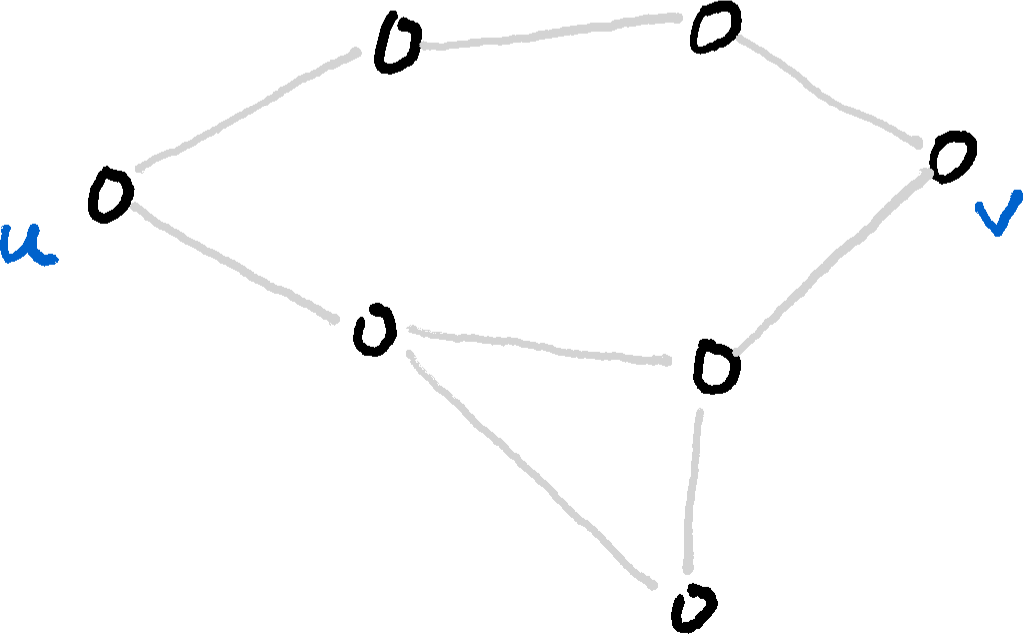
\includegraphics[width=0.6\textwidth]{graphics/L10_connectivity/twoconnected_graph.png}
  \caption[][1.5cm]{A graph of connectivity two. Removing any single vertex does not disconnect the graph, but there are obviously ways to remove two vertices to disconnect it.}
  \label{fig:twoconnected_graph}
\end{figure}

\begin{example}
  Every graph is zero-connected,\sidenote[][]{Unless you consider the ``empty graph'' $(\emptyset, \emptyset)$ to be a graph.} and every connected graph on at least two vertices is one-connected. $K_n$ is $n-1$-connected, as is a complete graph with one edge removed, and $K_{a,b}$ is $\min(a,b)$-connected. The graphs of connectivity zero are precisely the disconnected graphs and $K_1$.
\end{example}

\begin{definition}
  Let $G = (V,E)$ be a graph, and let $v, w \in V$ be two vertices and $A, B \subseteq V$ two sets of vertices.

  A set $X \subseteq V$ \emph{separates} $v$ from $w$ if $X \not\ni v, w$ and every path from $v$ to $w$ contains at least one vertex from $X$. We denote the minimum size of a set separating $v$ from $w$ by $\kappa(v,w)$.

  A set $X \subseteq V$ \emph{separates} $A$ from $B$ if every path from a vertex in $A$ to a vertex in $B$ contains at least one vertex of $X$. Notice that here we do not require $A$, $B$, and $X$ to be disjoint -- and in fact if $A\cap B\neq \emptyset$ we must have this intersection contained in $X$, or the lazy path starting and ending at the same vertex in $A\cap B$ would prevent separation.
\end{definition}

\begin{lemma}\label{lemma:connectivity_is_min_of_pairwise_connectivity}
  For a graph $G = (V,E)$ that is not a complete graph, we have
  $$\kappa(G) = \min_{\substack{u, v \in V\\u\sim v \not\in E}} \kappa(u,v).$$

  \begin{proof}
    Since $G$ is not complete, $\kappa(G)$ equals the minimum size of a set $X \subseteq V$ whose removal disconnects the graph.\sidenote[][]{Since it is not complete, there exists a pair of vertices without an edge between them. Removing all vertices but these two definitely disconnects the graph.} Let $X$ be a minimal such set, and so since $G[V \setminus X]$ is disconnected we can find $x_0$ and $y_0$ from different components, which are thus separated by $X$. So $\min_{x,y \in V} \kappa(x,y) \leq \abs{X} = \kappa(G)$.

    Conversely, let $x_0$ and $y_0$ be two non-adjacent vertices such that $\kappa(x_0, y_0)$ attains this minimum. Then there exists a separating set $X$ for $x_0$ and $y_0$ of size $\kappa(x_0, y_0) = \min_{x,y \in V: x\sim y \not\in E} \kappa(x, y)$. So in particular a set of this size suffices to disconnect $G$, and hence $\kappa(G) \leq \min_{x,y \in V: x\sim y \not\in E} \kappa(x, y)$.
  \end{proof}
\end{lemma}

\section{Menger's theorem}

We are now ready to show Menger's theorem, the content of which is that we could also have defined connectivity in terms of independent paths.

\begin{theorem}[Menger]\label{thm:menger_local}
  Let $G$ be a graph, and let $u$ and $v$ be two non-adjacent vertices of $G$. Then $\kappa(u,v)$, the minimum size of a set that separates $u$ and $v$, equals the maximum size of a set of independent paths from $v$ to $w$, where we say that two paths are independent if they share only their start and end point.

  \begin{proof}
    We will again use a clever flow network construction to prove this with the max-flow min-cut theorem.\sidenote[][]{So when I said in an earlier lecture that we were done applying this technique, I was obviously wrong.} The way we construct our flow network is to first replace every edge $x\sim y$ by two edges $x\to y$ and $y\to x$. Then, for every vertex $x$, except $u$ and $v$, we split it into two vertices $x_i$ and $x_o$, and replace every edge incoming to $x$ with one to $x_i$, and likewise every edge going out of $x$ with one going out of $x_o$. Finally, we add an edge from $x_i$ to $x_o$.

    \begin{figure}
      \centering
      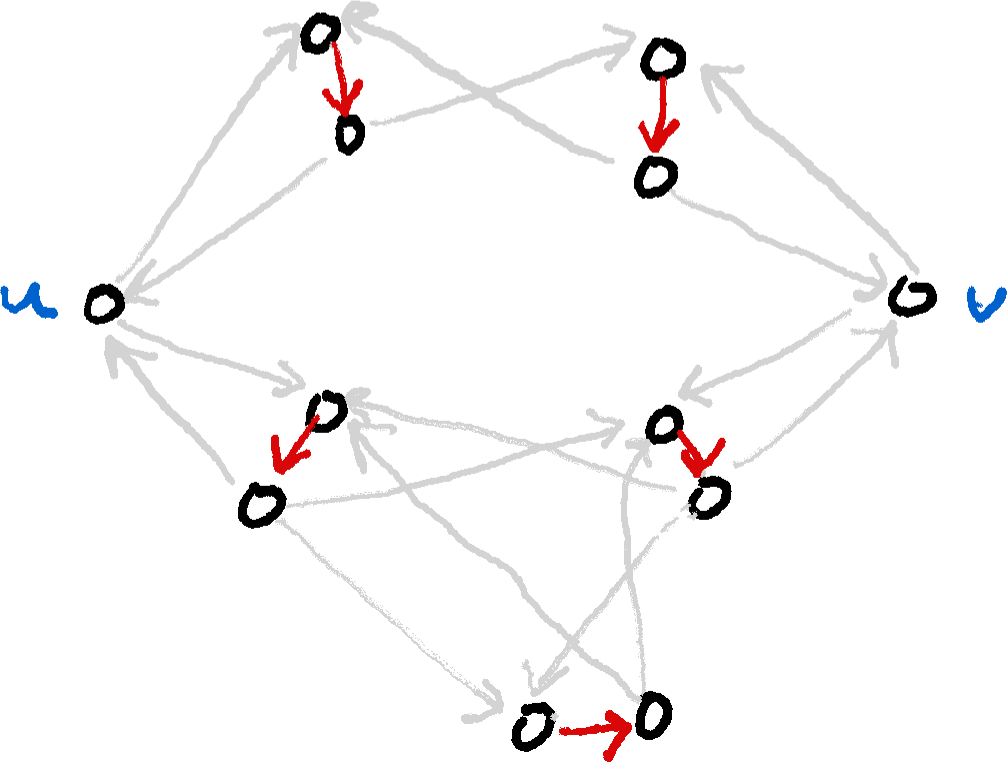
\includegraphics[width=0.6\textwidth]{graphics/L10_connectivity/menger_theorem_construction.png}
      \caption[][1.5cm]{The result of applying our flow network construction to the graph in Figure \ref{fig:twoconnected_graph}. Red edges have capacity one, grey edges have infinite capacity.}
      \label{fig:menger_thm_construction}
    \end{figure}

    We declare all edges to have infinite capacity, except for the ones from $x_i$ to $x_o$, which have capacity $1$.

    It is clear that an integer flow in this graph corresponds precisely to a set of independent paths from $u$ to $v$, since our construction with an edge of capacity one for each vertex means each vertex can only be used zero or one times. So a maximum flow corresponds to a maximum set of independent paths.

    Likewise, it is easy to see that a cut must, to have finite capacity, cut only through the edges of weight one, which correspond to vertices in the original graph, and their capacity is precisely the number of such vertices it cuts. So the capacity of a minimum cut is the minimum size of a set of vertices separating $u$ from $v$.

    So, by the max-flow min-cut theorem, the maximum number of independent paths equals the minimum size of a separating set.
  \end{proof}
\end{theorem}

At first glance, the following corollary looks like it should be entirely trivial, but it actually requires a little bit of work.

\begin{theorem}[Menger, global version]
  A graph is $k$-connected if and only if it contains $k$ independent paths between any two vertices.

  \begin{proof}
    Let $G = (V,E)$ be a graph. If $G$ has $k$ or fewer vertices, it is by definition not $k$-connected, and it is clearly impossible for there to be $k$ independent paths at all, since there are just too few vertices. Similarly, if $G$ is complete on more than $k$ vertices, we see easily that it is both $k$-connected and has the requisite number of independent paths. So we lose no generality in assuming $G$ is a non-complete graph on more than $k$ vertices.

    If $G$ is $k$-connected, then $\kappa(G) \geq k$ and hence $\kappa(u,v) \geq k$ for any two non-adjacent vertices $u$ and $v$ by Lemma \ref{lemma:connectivity_is_min_of_pairwise_connectivity}. By Menger's theorem, $u$ and $v$ are thus connected by at least $k$ independent paths.

    What remains to be shown is that we also have enough independent paths in the case where $u$ and $v$ \emph{are} adjacent. So assume for contradiction that there are at most $k-1$ independent paths from $u$ to $v$. After removing the edge $u \sim v$ from $G$ to get a graph $G'$, we are left with at most $k - 2$ independent paths from $u$ to $v$ in $G'$.

    Hence, by Menger's theorem, we can separate $u$ from $v$ by a set $X$ of size at most $k-2$ in $G'$. Since $G$ has more than $k$ vertices, there must be a vertex $w \in V \setminus (X \cup \{v,w\})$. Then this $w$ is separated by $X$ in $G'$ from either $u$ or $v$, say $u$. This however implies that $X \cup \{v\}$ separates $w$ from $u$, and $\abs{X \cup \{v\}} \leq k - 1$. This however contradicts the assumption that $G$ is $k$-connected.

    In the other direction, assume there exist at least $k$ independent paths between any two vertices. Then this holds in particular for any pair of non-adjacent vertices, and by assumption there is such a pair. So by Menger's theorem we have $\kappa(x,y)\geq k$ for all such pairs, and thus $\kappa(G) \geq k$ by Lemma \ref{lemma:connectivity_is_min_of_pairwise_connectivity}.
  \end{proof}
\end{theorem}

We could also have modified our proof of the ``local'' version of Menger's theorem to instead get this theorem:

\begin{theorem}[Menger]\label{thm:menger_setsep}
  Let $G = (V,E)$ be a graph, and let $A, B \subseteq V$ be sets of vertices. Then the minimum size of a set $X$ that separates $A$ from $B$ is equal to the maximum number of disjoint paths with one end in $A$ and the other end in $B$.
\end{theorem}

\begin{xca}
  Modify the proof of Theorem \ref{thm:menger_local} into a proof of Theorem \ref{thm:menger_setsep}.
\end{xca}

\section{The structure of two-connected graphs}

Determining what the one-connected graphs are is easy: They're the connected graphs. Can we give a similarly easy classification of the two-connected graphs? It turns out the answer is yes.

\begin{theorem}\label{lemma:structure_of_twoconnected_graphs}
  A finite\sidenote[][]{Do you actually need this assumption? If you enjoyed thinking about transfinite induction when we proved that Zorn's lemma implies \emph{all} graphs have spanning trees, you may enjoy trying to formalize a version of this without the finiteness assumption.} graph is two-connected if and only if it can be constructed from a cycle graph by successively adding paths to it, both of whose endpoints lie in the graph already constructed.

  \begin{proof}
    Every graph constructed in this way will be two-connected,\sidenote[][]{
      \begin{xca}
        Prove this. (Hint: Induction on the number of paths added.)
      \end{xca}
    } so what we need to show is that every two-connected graph can be constructed like this.

    Let us call a graph that can be constructed like this \emph{constructible}, and let $G$ be a two-connected graph. Clearly, $G$ must contain a cycle, since otherwise it'd be a tree or a forest, neither of which is two-connected. Thus, the set of constructible subgraphs of $G$ is non-empty, and it must in particular have a maximal (under the subgraph relation) element $H$.

    This $H$ must in fact be induced: If $x$ and $y$ were vertices of $H$ and $x\sim y$ an edge of $G$ but not of $H$, then this edge would be a path with both its endpoints in $H$, so we could add it to $H$ to get a larger constructible subgraph, which is a contradiction.

    So it remains to see that $H$ is spanning. So suppose it is not, and there exists some vertex in $G$ but not in $H$. Since $G$ is connected, there must in particular be such a vertex that is adjacent to $H$. Call it $y$, and let its neighbour in $H$ be $x$.
    
    Now, since $G$ is two-connected, removing the vertex $x$ does not disconnect it. Therefore, there still must exist a path $P$ connecting $y$ to some vertex in $H$. Then, however, this path $P$ together with the edge $y \sim x$ is a path with both endpoints in $H$, and so could be added to $H$ to get a larger constructible subgraph, a contradiction. So $H$ is spanning and induced, and thus $G = H$.
  \end{proof}
\end{theorem}

We know very well that we can divide a connected graph into its connected components. One way of phrasing this is that we can divide a zero-connected graph into parts that are one-connected. Can we also divide a one-connected graph into parts which are two-connected?

The answer to this question turns out to essentially be yes.\sidenote[][-1.5cm]{The same question for dividing a two-connected graph into three-connected components also turns out to have an affirmative answer, involving the amusingly named \emph{Tutte's angry theorem}. Unfortunately the pattern then breaks down, and you need special properties of the graph to be able to meaningfully talk about it having four-connected components and so on.}

\begin{definition}
  Let $G$ be a graph. A \emph{cutvertex} is a vertex whose removal increases the number of connected components of $G$. A \emph{bridge} is an edge whose removal increases the number of connected components of $G$. A \emph{block} is a maximal connected subgraph $H$ without a cutvertex in $H$,\sidenote[][]{By which we mean that $H$ considered as a graph on its own has no cutvertices, not that no vertex of $H$ is a cutvertex of $G$.} where we by maximal mean maximal with respect to the subgraph relation.
\end{definition}

Now, a block is not exactly the same thing as a two-connected subgraph, but it is very close to being that, as we shall see. It is clear that a two-connected graph has no cutvertices, so any two-connected subgraph is contained in a block -- and as we will see, it is contained in exactly one block.

To be able to prove this, we need the following innocuous-looking but in fact rather deep lemma:

\begin{lemma}\label{lemma:block_cycle_intersection}
  For any cycle $C$ in $G$, there is exactly one block intersecting it in more than one vertex.

  \begin{proof}
    Suppose $C$ is a cycle in $G$, and suppose for contradiction that $A$ and $B$ are two blocks both intersecting $C$ in multiple vertices. We claim that it is then the case that $C \cup A \cup B$ is a connected graph with no cutvertices, contradicting the maximality of $A$ and $B$.

    So suppose we remove a vertex $v$ from $C \cup A \cup B$. If $v \in C$, this clearly does not disconnect the graph. If $v\in A$, this does not disconnect $A$ itself, because $A$ had no cutvertices, and it cannot disconnect $A$ from the rest of $C \cup A \cup B$ since $A$ intersected $C$ in multiple vertices. The same argument of course works for $v \in B$. So we have shown that $C \cup A \cup B$ has no cutvertices.
  \end{proof}
\end{lemma}

What does a block look like? We can give a very precise classification.

\begin{lemma}\label{lemma:classification_of_blocks}
  Let $G$ be a graph, and $H$ a block of $G$. Then $H$ is an \emph{induced} subgraph of $G$, and three cases are possible:
  \begin{enumerate}
    \item $H$ contains just a single vertex of degree zero, an isolated vertex.
    \item $H$ consists of two vertices connected by an edge, and this edge is a bridge.
    \item $H$ is two-connected.
  \end{enumerate}

  Conversely, an isolated vertex always forms its own block, and the two vertices incident to a bridge always form a block.

  \begin{xca}
    Prove this. For the second case, use Lemma \ref{lemma:block_cycle_intersection}, and for the last, use Menger's theorem.
  \end{xca}
\end{lemma}

Our next question to ask is of course how the blocks may overlap. For the division of a graph into its connected components, they may of course not overlap at all, but for finding the twoconnected components we will have to allow a little bit of overlap. Fortunately, we can show that this is only ever a single vertex.

\begin{lemma}
  Let $G = (V,E)$ be a graph. Any two blocks of $G$ intersect in only zero or one vertices. If they intersect in a single vertex, that vertex must be a cutvertex of $G$.

  \begin{proof}
    Suppose for contradiction that $A$ and $B$ are two blocks of $G$, and $A \cap B \ni u,v$. It is clear by Lemma \ref{lemma:classification_of_blocks} that at least one of them has to be two-connected, say $A$.
    
    Since $A$ and $B$ are both connected, there exist paths $P$ and $P'$ connecting $u$ to $v$ in $A$ and $B$ respectively. If $u \sim v$ is not an edge, gluing together $P$ and $P'$ yields a cycle $C$ intersecting both $A$ and $B$ in the two vertices $u$ and $v$, contradicting Lemma \ref{lemma:block_cycle_intersection}.

    If $u\sim v \in E$, we could have been unlucky and picked both $P$ and $P'$ as the path consisting of just that one edge. However, we know $A$ is two-connected, so in $A$ there has to be two independent paths between $u$ and $v$. So we can just pick the one that is not the single edge, and then the union is again a cycle, yielding the first part of the lemma.

    For the second part the lemma, suppose $A$ and $B$ are two blocks intersecting in $v$, but $v$ is not a cutvertex of $G$. Then, pick a neighbours $a$ and $b$ of $v$ in $A$ and $B$ respectively.\sidenote[][]{These must exist, since otherwise one of the blocks would be of size one and thus a subset of the other, which is absurd.} Since $v$ is not a cutvertex of $G$, there exists a path in $G$ from $a$ to $b$ not using $v$. But then this path together with the path $a\, v\, b$ forms a cycle in $G$, intersecting $A$ in $a$ and $v$ and intersecting $B$ in $b$ and $v$ -- and this is a contradiction with Lemma \ref{lemma:block_cycle_intersection}.
  \end{proof}
\end{lemma}

\begin{corollary}\label{cor:noncutvertices_single_block}
  Any vertex $v$ of $G$ which is not a cutvertex is contained in exactly one block.
\end{corollary}

\begin{lemma}\label{lemma:edges_imply_same_block}
  Suppose $u$ and $v$ are two adjacent vertices. Then $u$ and $v$ belong to the same block.

  \begin{proof}
    If the edge $u \sim v$ is a bridge, then the set $\{u,v\}$ is itself a block by Lemma \ref{lemma:classification_of_blocks}, and so we are done.

    If it is not a bridge, then there is some path from $u$ to $v$ in $G$ not using the edge $u \sim v$, and so this path together with the edge forms a cycle. A cycle, however, is a graph with no cutvertices, so the subgraph it forms must sit within a maximal cutvertexless subgraph -- a block. So in particular $u$ and $v$ must share a block.
  \end{proof}
\end{lemma}

In fact, we can prove something much stronger than just that they intersect in nice ways -- we can create a graph whose vertices are the blocks and cutvertices of our original graph, and this graph will have a very nice structure.

\begin{figure}
  \centering
  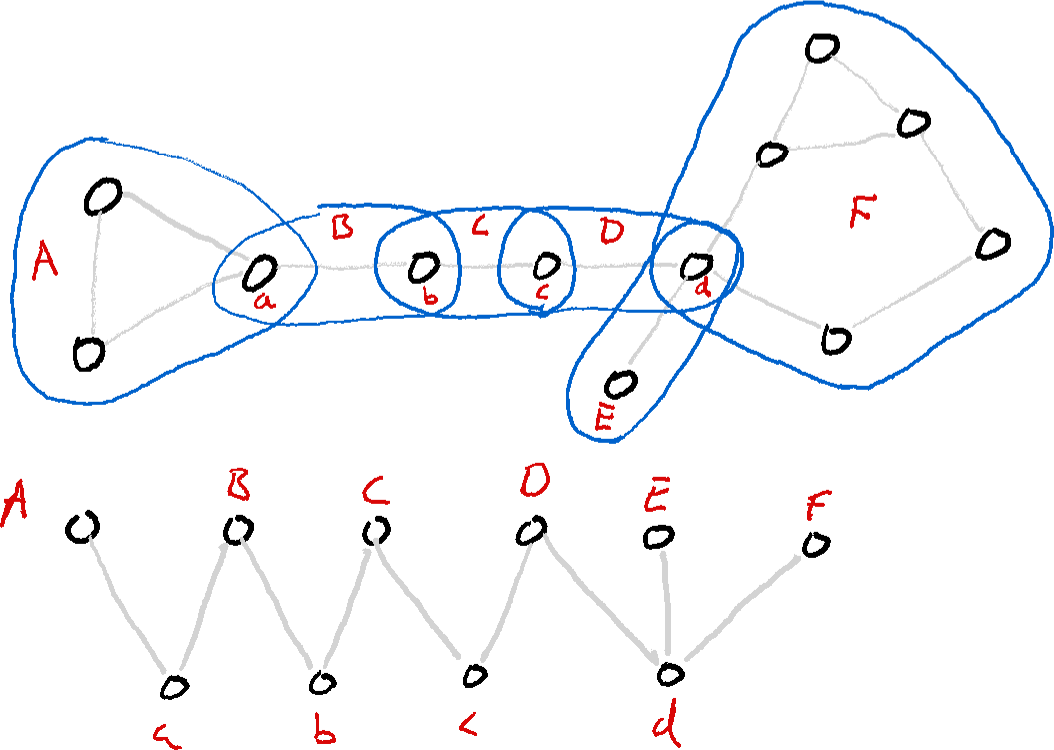
\includegraphics[width=0.75\textwidth]{graphics/L10_connectivity/graph_with_blockgraph.png}
  \caption[][0cm]{A graph, with its blocks circled in blue and labelled with red capital letters and its cutvertices labelled in red minuscule letters. Below, the corresponding block graph, with the same labeling.}
  \label{fig:graph_with_blockgraph}
\end{figure}

\begin{definition}
  Let $G$ be a graph, let $A$ be its collection of cutvertices, and $B$ its collection of blocks. The \emph{block graph} of $G$ is a bipartite graph with vertices $A \coprod B$, where an edge is drawn from $a\in A$ to $b\in B$ if $a$ is a vertex in $B$.
\end{definition}

\begin{lemma}\label{lemma:pathcorrespondence}
  Let $G$ be a graph and $B(G)$ its block graph. A walk in $G$ corresponds to a walk in $B(G)$ which intersects the same blocks and cutvertices in the same order. Likewise, for any walk in $B(G)$, there exists at least one walk in $G$ which corresponds to it.

  \begin{proof}[``Proof'']
    Look at Figure \ref{fig:pathcorrespondence} and convince yourself it is obvious.
  \end{proof}

  \begin{xca}
    Prove this rigorously.\sidenote[][]{I made an effort while writing the lecture notes, and it turned immediately into an unenlightening division into four cases.}
  \end{xca}

  \begin{figure}
    \centering
    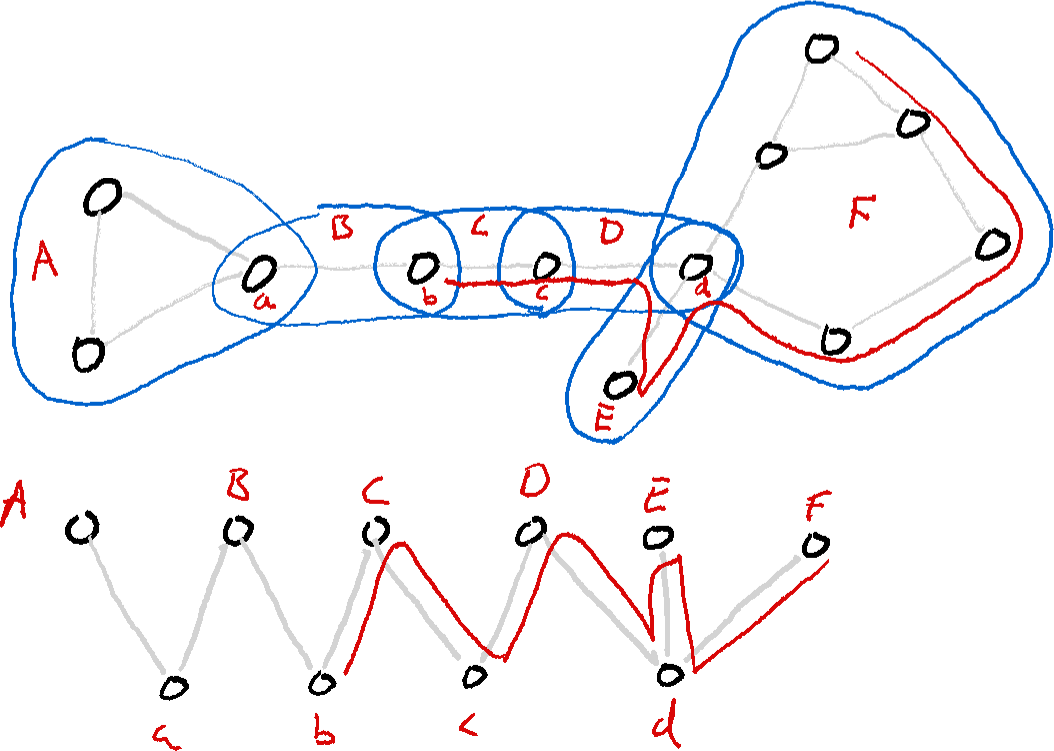
\includegraphics[width=0.75\textwidth]{graphics/L10_connectivity/pathcorrespondence.png}
    \caption[][0cm]{Figure \ref{fig:graph_with_blockgraph} with a walk drawn in in red on the graph, and its corresponding walk on the blackgraph, also in red.}
    \label{fig:pathcorrespondence}
  \end{figure}
  
  \begin{comment}
    Let $W = v_0\, e_1\, v_1\, \ldots\, v_{k-1}\, e_k\, v_k$ be a walk in $G$. If $v_0$ is a cutvertex, we of course start the walk in $B(G)$ at the vertex corresponding to this cutvertex. If it is not a cutvertex, it belongs to exactly one block by Corollary \ref{cor:noncutvertices_single_block}, so we can unambiguously pick this block as our starting point in $B(G)$.

    Then, we proceed in our construction of the path. Suppose we are currently at a vertex $v$ in our walk on $G$, and the next vertex in the walk $W$ is $w$. In our walk on $B(G)$, we are at a vertex $b$. There are four cases:
    \begin{enumerate}
      \item $b$ is on the block side, and $w$ is not a cutvertex. By Lemma \ref{lemma:edges_imply_same_block} $v$ and $w$ are in the same block, so we can stay at $b$ and advance our walk on $G$ by one step.
      \item $b$ is on the block side, and $w$ is a cutvertex. What we want to do here is to take a step from $b$ to $w$ in our walk on $B(G)$, but to be able to do this we must see that there is such an edge. Now, since $v$ and $w$ are adjacent, they are in the same block, and so $w$ is also in the block $b$, and so by our construction there is an edge $w \sim b$ in $B(G)$. So we can step to $w$ in both our walks, advancing both one step.
      \item $b$ is on the cutvertex side, and so corresponds to the cutvertex $v$, and $w$ is not a cutvertex. Since $w$ is not a cutvertex, it belongs to a single block, say $b'$. Since $v$ and $w$ are adjacent, $v$ also belongs to $b'$, and so there is an 
    \end{enumerate}

    \begin{enumerate}
      \item $v$ is not a cutvertex, and neither is $w$. Then Lemma \ref{lemma:edges_imply_same_block} tells us that $w$ must still be in the same block, and so in our walk on the block graph, we just stay put at our current block.
      \item $v$ is not a cutvertex, but $w$ is. Then, in our walk on $B(G)$, we walk to the vertex corresponding to $w$. To see that we can do this, we must see that there is an edge in $B(G)$ from the block of $v$ to the cutvertex $w$. Since $v$ and $w$ are adjacent, they are in the same block, and so there is an edge in $B(G)$ between the cutvertex $w$ and the block of $w$, which is also the block of $v$.
      \item $v$ is a cutvertex, but $w$ is not. Since $w$ is not a cutvertex, it belongs to only one block, and since $w$ and $v$ are adjacent, $v$ also belongs to this block. So by a similar argument as in the previous case, we can continue our walk in $B(G)$ from the cutvertex $v$ to the block of $w$.
      \item $v$ and $w$ are both cutvertices. Since they are adjacent, they must share a block, 
    \end{enumerate}
  \end{comment}
\end{lemma}

\begin{lemma}
  For any graph $G$, its block graph is a forest. If $G$ is connected, its block graph is a tree.

  \begin{proof}
    It is clear that if we prove the second assertion, the first follows by applying it to each connected component. So assume $G$ is connected.

    Now assume for contradiction that the block graph of $G$ contains a cycle. Since the block graph is bipartite, this cycle has to traverse at least two blocks of $G$. By Lemma \ref{lemma:pathcorrespondence}, this cycle in the block graph corresponds to a cycle in $G$, and this cycle must intersect two different blocks. If you think through the details of how the correspondence between walks in the graph and its block graph works,\sidenote[][]{Such as by doing the exercise to prove Lemma \ref{lemma:pathcorrespondence}.} it is clear that this cycle must intersect the blocks in at least two vertices, and so we have a contradiction with Lemma \ref{lemma:block_cycle_intersection}.
  \end{proof}
\end{lemma}

\section{Exercises}


%\bibliography{references}
%\bibliographystyle{plainnat}

\end{document}
